\documentclass[11pt]{article}
\usepackage{graphicx}
\usepackage{float}
\usepackage[utf8]{inputenc}
\usepackage[polish]{babel}
\usepackage[T1]{fontenc}
\graphicspath{ {images/} }
\begin{document}
\title{Struktury danych i złożoność obliczeniowa}
\author{Łukasz Wdowiak}
\begin{titlepage}
    \begin{center}


        \vspace*{-3cm}

        
\includegraphics[width=14cm]{images/image.png}

        \vspace*{2cm}
        \huge
        \textbf{Sprawozdanie z laboratorium nr 3 Mechanizmy SISD I SIMD}

        \vspace{0.5cm}


        \vspace{1.5cm}

        \textbf{Łukasz Wdowiak}

        \vspace{2cm}

        \vfill
        Prowadzacy: mgr inż. Tomasz Serafin \\
        \vspace{2cm}
        Wydział Informatyki i Telekomunikacji \\
        Informatyka Techniczna \\
        IV semestr\\




    \end{center}
\end{titlepage}
\section{Wykresy}
\begin{figure}[H]
    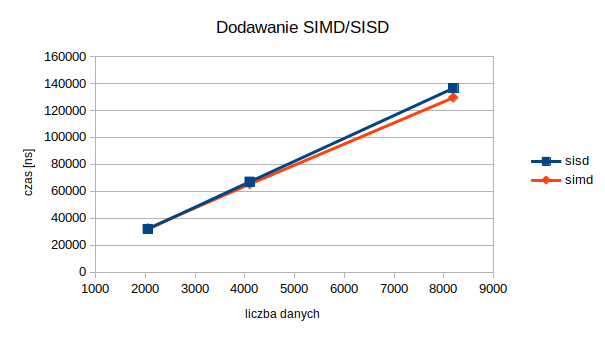
\includegraphics[width=13cm]{images/dodawanie.png}
    \caption{wykres średniego czasu dla dodawania}
\end{figure}
\begin{figure}[H]
    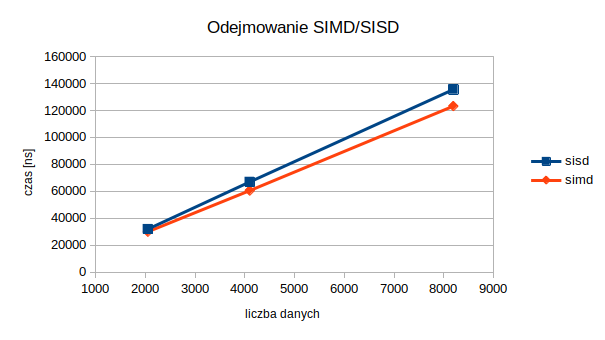
\includegraphics[width=13cm]{images/odejmowanie.png}
    \caption{wykres średniego czasu dla odejmowanie}
\end{figure}
\begin{figure}[H]
    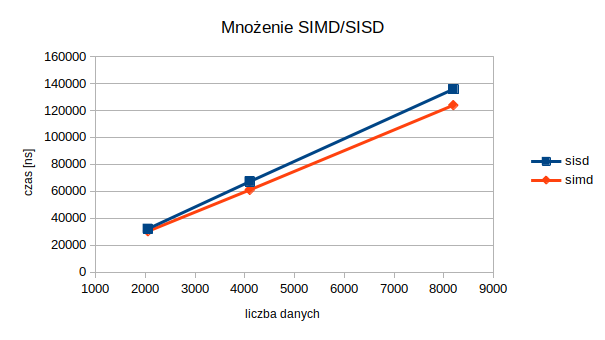
\includegraphics[width=13cm]{images/mnozenie.png}
    \caption{wykres średniego czasu dla mnożenia}
\end{figure}
\begin{figure}[H]
    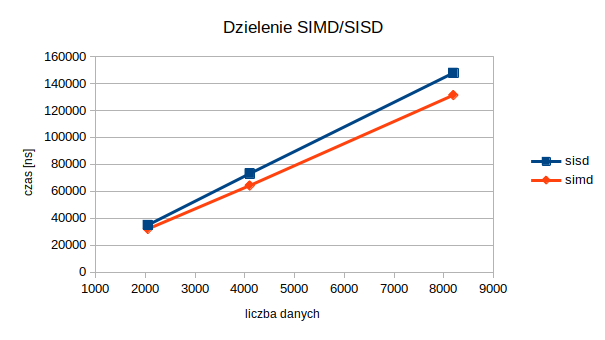
\includegraphics[width=13cm]{images/dzielenie.png}
    \caption{wykres średniego czasu dla dzielenia}
\end{figure}
\begin{figure}[H]
    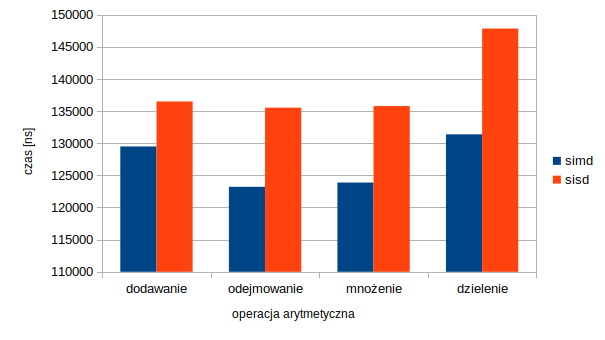
\includegraphics[width=13cm]{images/operacje.png}
    \caption{wykres średniego czasu od typu działania dla 8192 liczb}
\end{figure}
\begin{figure}[H]
    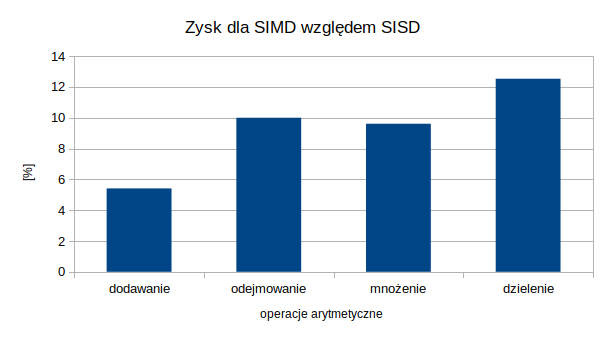
\includegraphics[width=13cm]{images/zysk.png}
    \caption{wykres zysku dla SIMD względem SISD dla 8192 liczb}
\end{figure}
\clearpage
\section{Przebieg pracy nad programem}
\begin{enumerate}
    \item      Stworzenie makefile
    \item      Stworzenie funkcji odpowiedzialnej za zapis do pliku
    \item      Research na temat SIMD
    \item      Stworzenie funkcji zapełniajacej wektory losowymi liczbami
    \item      Stworzenie funkcji dodawania/odejmowania/mnożenia/dzielenia dla SIMD
    \item      Research na temat SISD
    \item      Stworzenie funkcji zapełniajacej tablice losowymi liczbami
    \item      Stworzenie funkcji dodawania/odejmowania/mnożenia/dzielenia dla SISD
    \item      Napisanie funkcji testujacych
    \item      Urozmaicenie programu o parametry startowe (liczba powtórzeń, rozmiar tablicy)
\end{enumerate}
\section{Napotkane problemy}
\begin{itemize}
    \item  zapis składni assemblerowej w c++
    \item  zbyt losowe wyniki pomiarów przy małej ilości testów
\end{itemize}
\clearpage
\section{Kluczowe fragmenty kodu}
Przykładowa funkcja dodawania dla SIMD:
\begin{verbatim}
    double addVectorSIMD(Vector *v1, Vector *v2, Vector *result)
    {
        auto start = std::chrono::high_resolution_clock::now();
        __asm__ __volatile__(
            "movups (%0), %%xmm0\n"
            "movups (%1), %%xmm1\n"
            "addps %%xmm1, %%xmm0\n"
            "movups %%xmm0, (%2)\n"
            :
            : "r"(v1), "r"(v2), "r"(result)
            : "%xmm0", "%xmm1");
    
        auto end = std::chrono::high_resolution_clock::now();
        return std::chrono::duration_cast<std::chrono::nanoseconds>(end - start).count();
    }
\end{verbatim}
Czas wykonania operacji matematycznej jest mierzony za pomocą biblioteki chrono. Wstawka assemblerowa znajduje się w instrukcji\begin{verbatim}  __asm__ __volatile__ ();\end{verbatim} co oznacza mniej więcej tyle, że kod który teraz napiszemy będzie w assemblerze, a kompilator ma go nie optymalizować.
Kod assemblerowy przenosi wartość z argumentu pierwszego i drugiego do odpowiednio xmm0 i xmm1. Następnie użyta jest instrukcja dodania dwóch wektorów. Na sam koniec z xmm0 przenosimy wynik naszego dodawania do trzeciego argumentu naszej funkcji, czyli zmiennej result.
Pierwszy dwukropek jest wymagany jako dane wejściowe, drugi za dane wejściowe do kodu assemblera, trzecie za dane do zniszczenia.
\section{Opis uruchomienia programu}
Kompilacja programu:
\begin{verbatim}
    g++ -std=c++11 -o main main.cpp
\end{verbatim}
Program urachamiany jest z pomocą makefile. W celu uruchomienia programu należy wpisać w konsoli "make", a następnie "./main". W celu uruchomienia programu z parametrami należy wpisać "./main [liczba powtórzeń] [rozmiar tablicy]".
\section{Czym jest SIMD i SISD - rys historyczny}
\subsection{SISD (Single Instruction, Single Data)}
SISD to tradycyjny model obliczeń, w którym pojedyncza instrukcja jest wykonywana na pojedynczych danych. W takim przypadku procesor wykonuje kolejne instrukcje sekwencyjnie, przetwarzając jedną wartość danych na raz. To jest typowa architektura używana w większości konwencjonalnych procesorów.
\subsection{SIMD (Single Instruction, Multiple Data)}
SIMD to architektura, w której jedna instrukcja jest wykonywana jednocześnie na wielu zestawach danych. Oznacza to, że można równocześnie przetwarzać wiele danych przy użyciu jednej instrukcji, co może prowadzić do zwiększenia wydajności obliczeń. Procesory SIMD są zdolne do równoczesnego przetwarzania dużej liczby operacji, szczególnie przy obliczeniach równoległych, takich jak operacje na macierzach, przetwarzanie obrazów czy symulacje fizyczne.
\subsection{Rys historyczny}
SISD był dominującym modelem obliczeń na początku ery komputerów, gdzie jedna instrukcja była wykonywana sekwencyjnie na pojedynczych danych. W latach 60. i 70. XX wieku powstała architektura SIMD, umożliwiająca równoczesne przetwarzanie wielu danych. SIMD zyskało popularność w latach 80. i 90. dzięki rozwojowi technologii multimedialnych i  potrzeb przetwarzania danych wideo i dźwięku w czasie rzeczywistym. .
\section{Wnioski}
Z wykresów jasno wynika, że SIMD jest zdecydowanie szybsze. Zależność czasu wykonywania działań od liczby danych jest liniowa. Przy małej ilości testów tych samych wektorów (10 testów) niestety trudno zauważyć panujący schemat w różnicy pomiędzy SIMD, a SISD, gdyż czasy wykonywania operacji matematycznych mogą być różne, czasem wręcz losowe, z racji tego, że nie wiemy jakie operacje przeprowadza w tym momencie nasz system operacyjny. Dlatego też zwiększyłem liczby testów do 1000, co pozwala uzyskać bardziej wiarygodne wyniki.
Średni zysk SIMD wzgledem SISD dla róznych operacji wynosi około 10\%. SIMD zdecydowanie przyspiesza wykonywanie trudnych operacji matematycznych takich jak dzielenie.
\end{document}